\documentclass{article}
\usepackage{fullpage}
\usepackage{amssymb,amsmath,amsthm}
%\usepackage{bibentry}
\usepackage{natbib}
% to compile a camera-ready version, add the [final] option, e.g.:
% \usepackage[final]{nips_2017}
\title{Appendix}
\date{}

\usepackage[utf8]{inputenc} % allow utf-8 input
\usepackage[T1]{fontenc}    % use 8-bit T1 fonts
\usepackage{hyperref}       % hyperlinks
\usepackage{url}            % simple URL typesetting
\usepackage{booktabs}       % professional-quality tables
\usepackage{amsfonts}       % blackboard math symbols
\usepackage{nicefrac}       % compact symbols for 1/2, etc.
\usepackage{microtype}      % microtypography
\usepackage[utf8]{inputenc} % allow utf-8 input
\usepackage[T1]{fontenc}    % use 8-bit T1 fonts
\usepackage{hyperref}       % hyperlinks
\usepackage{url}            % simple URL typesetting
\usepackage{booktabs}       % professional-quality tables
\usepackage{amsfonts,amsthm}       % blackboard math symbols
\usepackage{nicefrac}       % compact symbols for 1/2, etc.
\usepackage{microtype}      % microtypography
\usepackage{MnSymbol}
\usepackage{color}
\usepackage{graphicx} % more modern
\usepackage{subfigure} 
\usepackage{natbib}
\usepackage{algorithm}
\usepackage{algpseudocode}
\usepackage{lineno}
\usepackage{thmtools,thm-restate}
\usepackage{xr}

%\linenumbers
\def\BIT{\begin{itemize}}
\def\EIT{\end{itemize}}
\def\BET{\begin{enumerate}}
\def\EET{\end{enumerate}}
\def\ra{$\:\rightarrow\:$}
\def\y{\mathbf{y}}
\def\x{\mathbf{x}}
\def\v{\mathbf{v}}
\def\u{\mathbf{u}}
\def\w{\mathbf{w}}
\def\s{\mathbf{s}}
\def\g{\mathbf{g}}
\def\h{\mathbf{h}}
\def\X{\mathbf{X}}
\def\RR{\mathbb{R}}
\def\ei{\varepsilon_i}
\def\ej{\varepsilon_j}
\def\T{\mathcal{T}}
\def\I{\mathcal{I}}

\def\op{{\rm op}}
\def\supp{{\rm Supp}}
\def\st{\text{s.t.}}
\newcommand\normop[1]{|||#1|||_{\infty}}
\newcommand\normbop[1]{|\!|\!|#1|\!|\!|_{\infty,2}}
\newcommand\normopop[1]{|\!|\!|#1|\!|\!|_{\rm op,\rm op}}
\newcommand\ve[1]{\varepsilon^{{\scriptscriptstyle#1}}}
\newcommand\sss[1]{{\scriptscriptstyle#1}}
\def\uI{U^{\sss{I}}}
\def\xxi{\zeta}






\def\A{\mathcal{A}}
\def\ga{\gamma_\mathcal{A}}
\def\Co{C^{\circ}}
\def\Coa{C^{\circ}_{\!\!\mathcal{A}}}
\def\Ca{C_{\!\mathcal{A}}}
\def\go{\gamma^{\circ}}
\def\goa{\gamma^{\circ}_{\A}}
\newcommand{\dt}[2]{\langle#1,#2\rangle}
\def\Olasso{\Omega_{\rm Lasso}} % Lasso norm
\def\Ogl{\Omega_{\rm GL}} % group Lasso norm
\def\Olgl{\Omega_{\rm LGL}} % latent group Lasso norm
\def\tr{\rm tr}
\newcommand\itgset[1]{[\!\![#1]\!\!]}
\def\RR{\mathbb{R}}
\def\EE{\mathbb{E}}
\newcommand{\tblue}[1]{\textcolor{blue}{#1}}
\newcommand{\tred}[1]{\textcolor{red}{#1}}
\newcommand\TODO[1]{\tblue{TODO: \texttt{#1}}}
%\newcommand\TODO[1]{}
\newcommand\OLD[1]{\tblue{#1}}
\newcommand\NEW[1]{\tred{#1}}
\def\st{\text{s.t.}}
\def\supp{\text{supp}}

\newtheorem{lemma}{Lemma}
\newtheorem{cor}{Corollary}
\newtheorem{prop}{Proposition}
\newtheorem{theorem}{Theorem}

\begin{document}
\maketitle
\appendix

\section{Proofs of section 3}

\begin{lemma} The polar gauge of $\Omega_{k,\succeq}$ of a symmetric $Y\RR^{p\times p}$ is
\begin{align}
\Omega_{k,\succeq}^{\circ}(Y):= \max_{I\in\mathcal{G}^p_k}\lambda^{+}_{max}(Y_{II})
\end{align}
\end{lemma}

\begin{proof}
\begin{align}
\Omega_{k,\succeq}^{\circ}(Y) 
&=\max_{\Omega_{k,\succeq}(X)\leq 1} \tr{Y^{\top}X}\\
&=\max_{c_i\geq 0, u_{i}, \|u_{i}\|_0=k, \|u_{i}\|_ 2=1 } \sum c_i u_{i}^{\top}Yu_{i} \quad s.t.  \sum c_i\leq 1\\
&=\max_{\|u\|_0=k, \|u\|_ 2=1 } u^{\top}Yu \\
&=\max_{I\in\mathcal{G}^p_k}\lambda^{+}_{max}(Y_{II})
\end{align}
\end{proof}

\begin{lemma} $\bar{\Omega}(M):=\inf\{\gamma\|A\|_{1}+\Omega_k(B)|M=A+B\}$ is an atomic norm and its dual is 
\begin{align*}
\gamma^{\circ}(Y)=\max\left(\frac{\|Y\|_{\infty}}{\gamma},\Omega_{k,\succeq}^{\circ}(Y)\right)
\end{align*}
\end{lemma}

\begin{proof}
$\ell_1$ is an atomic norm with atomic set $\mathcal{A}_{\ell_{1}}=\{\pm e_i e_j^{\top}\}$ where $e_i$ is the canonical basis of $\RR^p$. $\Omega_{k,\succeq}$  is an atomic norm with atomic set $\mathcal{A}_{k,\succeq}=\{uu^{\top}  :  u\in\RR^{p} \quad \|u\|_0 \leq k, \|u\|_2 = 1\}$. We can write,
$$
\bar{\Omega}(M)= \inf \big\{\|a\|_1+\|b\|_1 \quad s.t. \quad M=\sum_{j} b_j B_{j} + \sum_{i} a_i A_{i}, \quad c_i\in \RR^{+}\quad B_j\in\frac{1}{\gamma}\mathcal{A}_{\ell_{1}} \quad A_i\mathcal{A}_{k,\succeq} \big\}
$$
so $\bar{\Omega}$ is an atomic norm with atomic set $\frac{1}{\gamma}\mathcal{A}_{\ell_{1}}\cup\mathcal{A}_{k,\succeq}$. The dual norm writes
\begin{align}
\gamma^{\circ}(Y)
& = \max_{X\in\frac{1}{\gamma}\mathcal{A}_{\ell_{1}}\cup\mathcal{A}_{k,\succeq}} \tr{Y^{\top}X}\\
& =\max\left(\max_{B\in\frac{1}{\gamma}\mathcal{A}_{\ell_{1}}}\tr{Y^{\top}B}, \max_{A\in\mathcal{A}_{k,\succeq}}\tr{Y^{\top}A}\right)\\
& =\max\left(\frac{1}{\gamma}\max_{\tilde{B}\in\mathcal{A}_{\ell_{1}}}\tr{Y^{\top}\tilde{B}}, \max_{\tilde{A}\in\mathcal{A}_{k,\succeq}}\tr{Y^{\top}\tilde{A}}\right)\\
& =\max\left(\frac{\|Y\|_{\infty}}{\gamma},\Omega_{k,\succeq}^{\circ}(Y)\right)
\end{align}
%
%
%& =\max\left(\frac{\|Y\|_{\infty}}{\gamma},\Omega_{k,\succeq}^{\circ}(Y)\right)
\end{proof}

%---------------------------------------------------------------------------------------
%---------------------------------------------------------------------------------------
%---------------------------------------------------------------------------------------
%---------------------------------------------------------------------------------------
%---------------------------------------------------------------------------------------
%---------------------------------------------------------------------------------------
%---------------------------------------------------------------------------------------
%---------------------------------------------------------------------------------------
%---------------------------------------------------------------------------------------
%---------------------------------------------------------------------------------------
%---------------------------------------------------------------------------------------
%---------------------------------------------------------------------------------------
%---------------------------------------------------------------------------------------
%---------------------------------------------------------------------------------------
%---------------------------------------------------------------------------------------

%\subsection*{Notations}
%In this appendix, we will use two different several norms on matrices, the $\ell_\infty$ norm of the vectorized matrix, also known as the max-norm in the matrix case that we will denote with $\|\cdot\|_{\infty}$.
\section{Abstract lemmas on collections of incoherent subspaces}
The following lemma generalizes a classical upper bound on $|||A^{-1}|||_{\infty}$ discussed in \citet{varga1976diagonal} for diagonally dominant matrices, where $|||\cdot|||_{\infty}$ is the operator $\ell_\infty$ norm (equal to the maximal $\ell_1$-norm of all rows), not to be confused with the 
$\ell_\infty$ norm of the vectorized matrix, also known as the max-norm that we denote with $\|\cdot\|_{\infty}$ throughout the paper.

\begin{lemma}
\label{lem:gbdd}
Let $A=(A_{ij})$ a matrix defining a linear operator from $\RR^{r_1} \times \ldots \times \RR^{r_m}$ to itself, with $A_{ii}=Id_{r_i}$. Consider a collection of norms $\omega_i$ each defined on $\RR^{r_i}$
and define $\omega(x)=\max_i \omega_i(x_i)$. Define the matrix operator norm $|||A|||_{\omega,\omega}=\max_{x:\omega(x)\leq 1} \omega(Ax)$ and consider the quantities:
$\xxi_{ij}=\max_{x_j:\omega_j(x_j) \leq 1} \omega_i(A_{ij}x_j)$.
Then if 
$$\alpha:=1-\max_{i} \sum_{j \neq i} \xxi_{ij}$$ is such that $\alpha >0$, then $A$ is invertible and $|||A^{-1}|||_{\omega,\omega}< \frac{1}{\alpha}$.
\end{lemma}
\begin{proof}
Consider a vector $x$ and assume that $i=\text{arg} \max_{k} \omega_k(x_k)$ then

\begin{eqnarray*}
\alpha \, \omega(x) =\alpha \, \omega_i(x_i) &\leq & \omega_i(x_i) -\sum_{j\neq i} \xxi_{ij}  \, \omega_i(x_i) \leq \omega_i(x_i) -\sum_{j\neq i} \xxi_{ij}  \, \omega_j(x_j)\\
&\leq& \omega_i(Id_{r_i} x_i) -\sum_{j\neq i} \, \omega_i(A_{ij} x_j)
\leq \omega_i(A_{ii} x_i) -\omega_i \big ( \sum_{j\neq i} A_{ij} x_j \big )\\
&\leq&\omega_i \big ( \sum_{j=1}^p A_{ij} x_j \big )
\leq\omega_i (A_{i\cdot}x)=\omega(A x)\\
\end{eqnarray*}

Since this inequality is true for all $x$, it proves that for all $x$, $Ax\neq0$ which entails that $A$ is invertible.
Furthermore,
$$\alpha\leq \inf_{x\neq 0} \frac{\omega(A x)}{\omega(x)}=\inf_{y\neq 0} \frac{\omega(y)}{\omega(A^{-1}y)},$$
given that $y$ is invertible and so $\sup_{y \neq 0}\frac{\omega(A^{-1}y)}{\omega(y)}\leq \frac{1}{\alpha}$ which is the result we want
\end{proof}

\begin{lemma}
\label{lem:two}
In the particular case where there are only two blocks in the previous lemma if $\xxi_{12}\xxi_{21}<1$ then $A$ is invertible and we have $$|||A^{-1}|||_{\omega,\omega} \leq \frac{1+\max(\xxi_{12},\xxi_{21})}{1-\xxi_{12}\xxi_{21}}.$$
\end{lemma}
\begin{proof}
Indeed letting $B:=A_{12}$ so that 
$$A=
\begin{bmatrix}
I & B\\
B^\top & I
\end{bmatrix}
$$
we have that $A$ is invertible if $A^\top A \succ I$, and, in that case
$$A^{-1}=A D \quad \text{with} \quad D:= 
\begin{bmatrix}
(I-BB^\top)^{-1} & 0\\
0 & (I-B^\top B)^{-1}
\end{bmatrix}
$$
Similarly as in the previous proof, letting $\alpha':=1-\xxi_{12} \xxi_{21}$, and using that $\omega_1(BB^\top x_1) \leq \xxi_{12} \omega_2(B^\top x_1) \leq  \xxi_{12} \xxi_{21} \omega_2(x_1),$ 
we have
$$\alpha' \omega_1(x_1) \leq \omega_1(x_1)- \xxi_{12} \xxi_{21} \omega_1(x_1) \leq \omega_1(x_1)- \omega_1(BB^\top x_1) \leq \omega_1 \big ( (I-BB^\top) x_1 \big ).$$
so that if $\alpha'>0$ then $I-BB^\top$ is invertible and so are  $I-B^\top B$,$D$ and $A$. Moreover, we have $|||D|||{\omega,\omega} \leq \frac{1}{\alpha'}$. Finally, $\omega_1(x_1-Bx_2)\leq \omega_1(x_1)-\omega_1(Bx_2) \leq (1+\xxi_{12}) \omega_1(x_1)$ and symmetrically, $\omega_2(x_2-B^\top x_1) \leq (1+\xxi_{21}) \omega_2(x_2)$, so that $|||A|||_{\omega,\omega} \leq 1+\max(\xxi_{12},\xxi_{21})$ and the result follows using that $|||A^{-1}|||_{\omega,\omega} \leq |||A|||_{\omega,\omega} \, |||D|||_{\omega,\omega}$.
\end{proof}


\begin{cor}
\label{cor:small_x}
Let $\T_i$ a collection of subspaces of $\RR^d$ equipped each with a norm $\Omega_i$. For all $i$, let $\eta_i,\varepsilon_i \in \T_i$ such that
$\Omega_i(\eta_i) \leq \epsilon$. Let $T_i \in \RR^{d \times r_i}$ a matrix whose columns form an orthogonal basis of $\T_i$.  If $\xxi_{ij}(\T_i,\T_j):=\max_{u_j \in \T_j,\: \Omega_j(u_j) \leq 1} \Omega_i(P_i u_j)$, with $P_i:=T_iT_i^\top$ the projector on the subspace $\T_i$. Define $\alpha$ to be the quantity
$$\alpha=1-\max_{i} \sum_{j\neq i} \xxi_{ij}(\T_i,\T_j).$$
Then if, for all $i$, we have that 
$\eta_i=\sum_{j=1}^m P_i\varepsilon_j,$
 and if $\alpha>0$, then the $(\varepsilon_i)_{1 \leq i \leq m}$ are uniquely defined and for all $i,\: \Omega_i(\varepsilon_i) \leq \frac{\epsilon}{\alpha}$.
\end{cor}
\begin{proof}
If $\eta_i, \varepsilon_i \in \T_i$ then there exist unique $b_i$ and $x_i$ in $\RR^{r_i}$ such that $\eta_i=T_i b_i$ and $\varepsilon_i=T_i x_i$.
This entails that the equation $\eta_i=\sum_{j=1}^m P_i\varepsilon_j,$ is equivalent to $b_i=\sum_{j=1}^m T_i^\top T_j x_j$. As a consequence,
if $T:=[T_1,\ldots,T_m]$, let $A:=T^\top T$, then the system of equations relating $\eta:=(\eta_1;\ldots;\eta_m)$ to $x:=(x_1,\ldots,x_m)$ is equivalent to $\eta=A x$.
Moreover if $\omega_i(x_i):=\Omega_i(T_i x_i)$ then the quantities $\xxi_{ij}(\T_i,\T_j)$ and $\alpha$ defined in this corollary match respectively the quantities $\xxi_{ij}$ and $\alpha$ defined from $A$ in Lemma~\ref{lem:gbdd}. By applying the lemma, we thus get that $A$ is invertible and that
$$\max_i\Omega_i(\varepsilon_i)=\max_i \Omega_i(T_i x_i)=\omega(x)=\omega(A^{-1}b)\leq \frac{1}{\alpha} \omega(b)= \frac{1}{\alpha} \max_{i} \Omega_i(T_i b_i)= \frac{1}{\alpha}\max_i\Omega_i(\eta_i) \leq  \frac{\epsilon}{\alpha}.$$
\end{proof}

\begin{cor}
\label{cor:small_x_two}
In the case of two blocks the conclusion of Corollary~\ref{cor:small_x} hold for $\alpha=\frac{1-\xxi_{12}\xxi_{21}}{1+\max(\xxi_{12},\xxi_{21})}$.
\end{cor}
\begin{proof}
This follows from using the bound on $|||A^{-1}|||_{\omega,\omega}$ from Lemma~\ref{lem:two} in the proof of Corollary~\ref{cor:small_x}
\end{proof}


\begin{cor}
\label{cor:main}
Let $\T_i,T_i,P_i,\Omega_i, \xxi_{ij}(\T_i,\T_j)$ and $\alpha$ be defined as in Corollary~\ref{cor:small_x}. Let $(q_i)_{1\leq i \leq m}$ be a given collection of vectors in $\RR^d$ with $q_i \in \T_i$. 
Let $\eta_i=P_i \sum_{j \neq i} q_j$.
Assume that
\BIT
\item the $q_i$ are sufficiently close to orthogonal to the subspaces $\T_j$ for $j \neq i$, so that there exists $\epsilon>0$ with $\max_{i} \Omega_i(\eta_i) \leq \epsilon$.
\item we have $\alpha>0$.
\EIT
Then,  in $\text{span}(\T_1,\ldots,\T_m)$, the set of equations \{$P_i q=q_i, \: \forall i$\} admits a unique solution of the form $q=\sum_{i=1}^m (q_i+\varepsilon_i)$ with $\varepsilon_i$ in $\T_i$ and $\max_i\Omega_i(\varepsilon_i) \leq  \frac{\epsilon}{\alpha}$.
\end{cor}
\begin{proof}
If $q \in \text{span}(\T_1,\ldots,\T_m)$, then $q$ can be written under the form $q=\sum_{i=1}^m (q_i+\varepsilon_i)$ with $\varepsilon_i$ in $\T_i$ and $q$ solves the previous collection of equation if and only if for all $i$
$$q_i=P_i q=q_i +P_i \sum_{j \neq i} q_j+ P_i \sum_{j} \ej.$$
so that if $\eta_i:=-P_i \sum_{j \neq i} q_j$, then $\eta_i$ must satisfy $\eta_i= P_i \sum_{j} \ej$. Furthermore, $\eta$, $\varepsilon$ and the subspace $\T_i$ equipped with the norms $\Omega_i$ together satisfy the conditions of the previous corollary which proves the existence of a solution $q$ of the given form and the announced inequality.
\end{proof}

Note that requiring that $\alpha>0$ in the previous lemma corresponds to a way of quantifying that the subspaces $\T_i$ are \emph{sufficiently incoherent}.

\begin{cor}
\label{car:main_two}
In the case of two blocks, the conclusion of Corollary~\ref{cor:main} holds for $\alpha=\frac{1-\xxi_{12}\xxi_{21}}{1+\max(\xxi_{12},\xxi_{21})}$.
\end{cor}
\begin{proof}
This follows from the same proof as in Corollary~\ref{cor:main} but using Corollary~\ref{cor:small_x_two} instead of Corollary~\ref{cor:small_x}.
\end{proof}

\begin{lemma}
\label{lem:zero_inter}
In the case of two subspaces let $\alpha=\frac{1-\xxi_{12}\xxi_{21}}{1+\max(\xxi_{12},\xxi_{21})}$. Otherwise let $\alpha=1-\max_{i} \sum_{j\neq i} \xxi_{ij}(\T_i,\T_j).$

If $\alpha>0$, then $\forall i, \: \T_i \cap \text{span}\big ( (\T_j)_{j\neq i}\big) =\{0\}$.
\end{lemma}
\begin{proof}
Assume, by contradiction that there exist $(u_i)_{1\leq i\leq m}$, with $u_i \in \T_i$ and
$\sum_{j=1}^m u_j=0$. Then, if $\Omega_i(u_i)=\Omega(u):=\max_j \Omega_j(u_j)$, we have 
$$\Omega(u)=\Omega_i(u_i)=\Omega_i(-P_i u_i)=\Omega_i \big ( \sum_{j \neq i} P_i u_j \big ) \leq \sum_{j \neq _i} \Omega_i(P_i u_j) \leq \sum_{j \neq _i} \xxi_{ij} \Omega_j(u_j) \leq (1-\alpha) \Omega(u).$$ Since $\alpha>0$ this entails $\Omega(u)=0$ and so $u_i=0$ for all $i$. 
\end{proof}




\section{Application to low rank +sparse matrix decompositions}
\subsection{General notations}
We consider several type of subspaces
$$\bar{\T}_I:=\{M \in \RR^{p \times p}\mid  M=M^\top, \: \supp(M)\subset I \times I\},$$
$$\T_I(U):=\{M \in \bar{\T}_I\mid \: M=UX^\top+XU^\top,\: X \in \RR^{\text{rank}(U) \times p} \},$$
Let $\T^c_I(U)$ denote the orthogonal complement\footnote{Note in particular that it is not the orthogonal complement in the entire space.} of $\T_I(U)$ in $\bar{\T}_I$. 
$$\T(U):=\T_{[\![p]\!]}(U)\quad \text{and} \quad \T_s(A)=\{M \in \RR^{p \times p}\mid  \: M=M^\top, \: \supp(M)\subset \supp(A)\}.$$
The projections on the corresponding subspaces are $\mathcal{P}_{\T_s(A)}(M)=M_S$ and $\mathcal{P}_{\T_I(U)}(M)=\mathcal{P}_{U}(M_{II})$ with $$\mathcal{P}_U(M):=M-(I-UU^\top)M(I-UU^\top).$$


\subsection{Convex low rank+ sparse decomposition}
We first show that our assumptions yields results that are different than the one obtained in \citet{chandrasekaran2011rank} and potentially sharper.
\begin{cor}
Consider a matrix $M=A^*+B^*$ as in \citet{chandrasekaran2011rank}. Let 
\begin{eqnarray*}
\mu:=\mu(A^*)&:=&\max \{ \|N\|_{\op} \mid N \in \T(A^*), \|N\|_{\infty} \leq 1\}\\
 \xi:=\xi(B^*)&:=&\max \{ \|N\|_{\infty} \mid N \in \T(B^*), \|N\|_{\op} \leq 1 \}\\
\mu':=\zeta(\T(B^*),\T(A^*))&:=&\max \{ \|\mathcal{P}_{\T(B^*)}(N)\|_{\op} \mid N \in \T(A^*), \|N\|_{\infty} \leq 1\} \\ 
\xi':=\zeta(\T(A^*),\T(B^*))&:=&\max \{ \|\mathcal{P}_{\T(A^*)}(N)\|_{\infty} \mid N \in \T(B^*), \|N\|_{\op} \leq 1 \}\\
\epsilon&:=&\max \big (\|\mathcal{P}_{\T(B^*)}(\gamma \text{sign}(A^*))\|_{\op}, \gamma^{-1}\|UV^\top\|_{\infty} \big ).
\end{eqnarray*}

Let $\alpha:=\frac{1-\mu'\xi'}{1+\max(\gamma \mu',\frac{1}{\gamma} \xi')}$. Then if $\max(\mu,\xi) (1+\frac{\epsilon}{\alpha})<1$, the solution of the optimization problem
$$\min_{A+B=M} \gamma \|A\|_{1}+\|B\|_{\op}$$
has a unique solution which is $(A^*,B^*)$. 
\end{cor}
\begin{proof}
The proof follows the reasoning in \citet{chandrasekaran2011rank} and requires to prove that $\T_s(A^*)\cap \T(B^*)=\{0\}$ and that there exists a subgradient $Q$ of the form $Q=\gamma sign(A^*)+UV^\top+\ve{A}+\ve{B}$, where $B^*=USV^\top$
is the singular value decomposition of $B^*$, and with $\ve{A} \in \T_s(A^*)$,  $\ve{B} \in \T(B^*)$,
such that $\mathcal{P}_{\T_s(A^*)}(Q)=\gamma sign(A^*)$, $\mathcal{P}_{\T(B^*)}(Q)=UV^\top$, $\|\mathcal{P}_{\T_s(A^*)^\bot}(Q)\|_{\infty} <\gamma$ and  $\|\mathcal{P}_{\T(B^*)^\bot}(Q)\|_{\op} <1$. The fact that $\T_s(A^*)\cap \T(B^*)=\{0\}$ follows from applying Lemma~\ref{lem:zero_inter} to the spaces $\T_1=\T_s(A^*)$ and $\T_2=\T(B^*)$ equipped respectively with the norms $\Omega_1=\frac{1}{\gamma}\|\cdot\|_{\infty}$ and $\Omega_2=\|\cdot\|_{\op}$. The fact that and adequate $Q$ exists follows from applying Corollary~\ref{cor:main} with the same subspaces which yields that
$\|\ve{A}\|_{\infty} \leq \gamma \frac{\epsilon}{\alpha}$ and $\|\ve{B}\|_{\op} \leq \frac{\epsilon}{\alpha}$ so that 
$$\|\mathcal{P}_{\T_s(A^*)^\bot}(Q)\|_{\infty}=\|\mathcal{P}_{\T_s(A^*)^\bot}(UV^\top+\ve{B})\|_{\infty}\leq \|UV^\top+\ve{B}\|_{\infty} \leq \gamma \mu \|UV^\top+\ve{B}\|_{\op} \leq \gamma \mu (1+\epsilon/\alpha).$$
$$\|\mathcal{P}_{\T(B^*)^\bot}(Q)\|_{\op}=\|\mathcal{P}_{\T_s(A^*)^\bot}(\gamma sign(A^*)+\ve{A})\|_{\op}\leq \|\gamma sign(A^*)+\ve{A}\|_{\op} \leq \xi \|sign(A^*)+\gamma^{-1}\ve{A}\|_{\infty} \leq  \xi (1+\epsilon/\alpha).$$
\end{proof}

Note that $\mu'\leq \mu$ and $\xi'\leq \xi$ but that $\mu'$ and $\xi'$ are potentially smaller. Also $\epsilon \leq \max(\gamma \mu, \gamma^{-1}\xi)$ but since $\epsilon$ is a bound that holds for the very specific elements $sign(A^*)$ and $UV^\top$ of the tangent spaces $\T(A^*)$ and $\T(B^*)$ and not uniformly over all the tangent space like $\mu', \xi',\mu$ and $\xi'$ it is reasonable to assume that it can be much smaller. 

\subsection*{Low rank with sparse factors + sparse decomposition.}
Let 
\begin{eqnarray*}
\xxi(\T_s(S),\T_J(V))&=&\max \{ {\|M_S\|_\infty} \mid M \in \T_J(V), \: \|M\|_{\op}\leq 1\}\\
\xxi(\T_I(U),\T_s(S))&=&\max \{ {\|\mathcal{P}_{U}(M_{II})\|_{\op}} \mid M \in \T_s(S), \: \|M\|_{\infty}\leq 1\}\\
\xxi(\T_I(U),\T_J(V))&=&\max \{ {\|\mathcal{P}_{U}(M_{II})\|_{\op}} \mid  M \in \T_J(V), \: \|M\|_{\op}\leq 1\}\\
\xi(\T_J(V))&=&\max \{ {\|M\|_\infty} \mid M \in \T_J(V), \: \|M\|_{\op}\leq 1\}\\
\mu_I(\T_s(S))&=&\max \{ {\|M_{II}\|_\op} \mid M \in \T_s(S), \: \|M\|_{\infty}\leq 1\}\\
\end{eqnarray*}

\begin{theorem}
\label{theo:two}
If $M^*=S^*-L^*$ with $$L^*=\sum_{I \in \mathcal{I}} L^{\sss{I}},  \quad \supp(L^{\sss{I}}) \subset I \times I$$ for $\I \subset \mathcal{G}^p_k$ %(where $\mathcal{G}^p_k$ is the collection of all subsets of size $k$ of $[\![p]\!]$)
and $L^{\sss{I}}=U^{\sss{I}} D^{\sss{I}} {U^{\sss{I}}}^\top$ the eigenvalue decomposition of $L^{\sss{I}}$.

Let $$\mu'_I=\xxi(\T_I(U),\T_s(S)), \quad  \xi'_I :=\xxi(\T_s(S),\T_I(U)), \quad \mu_I:=\mu_I(\T_s(S)) , \quad \xi_I:=\xi(\T_I(U)),$$
and 
$$\alpha_I:=\frac{1-\mu'_I\xi'_I}{1+\max(\gamma \mu'_I,\frac{1}{\gamma} \xi'_I)} \qquad \text{and} \qquad \epsilon_I :=\max \big (\|\mathcal{P}_{\T_I(\uI)}(\gamma \text{sign}(S^*))\|_{\op}, \gamma^{-1}\|\uI {\uI}^\top\|_{\infty} \big ).$$

Assume that for all $(I,I') \in \I \times \I, I \cap I'=\varnothing$. If $$\displaystyle\max_{I \in \I} \max(\mu_I,\xi_I) (1+\frac{\epsilon_I}{\alpha_I})<1, \quad \displaystyle \max_{J \in \mathcal{G}^p_k} \lambda_{\max}^+\big (S^*_{\bar{I}^c \cap (J \times J)} \big ) <1$$ %\quad 
%\text{and}  \quad \max_{J \in \mathcal{G}^p_k, J \neq I}\lambda_{\max}^+(\uI_J{\uI_J}^\top)<1,$$
with $\displaystyle \bar{I}=\bigcup_{I \in \I} I \times I$,
then the  decomposition given by $\big (S^*,(D^{\sss{I}} \big)_{I \in \I},(\uI)_{I \in \I} \big )$ is solution to the optimization problem $$\displaystyle \min \gamma \|S\|_1+\Omega_{k,\succeq}(L) \quad \text{\st} \quad M=S+L.$$
\end{theorem}
\begin{proof}
We follow the general proof scheme of \citet{chandrasekaran2011rank}. The optimization problem admits the unique announced solution if it satisfies first order gradient condition in the sense that there exists a subgradient $Q \in \RR^{p \times p}$ that satisfies the following conditions
\BET
\item[(i)] for all any $M^\sss{s} \in \T_s(S^*)$ and $(M^{\sss{I}})_{I \in \I}$ with $M^{\sss{I}} \in \T_I(\uI)$, $M^\sss{s}+\sum_{I \in \I} M^{\sss{I}}=0 \: \Rightarrow \: (M^{\sss{I}}=0, \:I \in \I)$.
\item[(ii)] for all $I \in \I,\:\mathcal{P}_{\T_I(\uI)}(Q)=\uI{\uI}^\top$
\item[(iii)] $\mathcal{P}_{\T_s(S^*)}(Q)=\gamma sign(S^*)$
\item[(iv)] for all $I \in \I,\:\lambda_{\max}^+\big (\mathcal(P)_{\T_I^c(\uI)}(Q) \big )<1$
\item[(v)] $\|Q_{S^c}\|_{\infty}<\gamma$
\item[(vi)] for all $J \in \mathcal{G}^p_k \backslash \I, \: \lambda_{\max}^+(Q_{JJ})\leq 1$
\EET
We now prove the different statements. As a consequence of the assumption that $I \cap I'=\varnothing, (I,I') \in \I \times \I,$ the space of symmetric squared matrices can be written as the direct sum of the spaces $(\bar{\T}_I)_{I \in \I}$ and of the space $\T^c:=\{M \in \RR^{p \times p} \mid  M=M^\top, \: M_{\bar{I}}=0\}$. Which entails that part of the properties to prove can be shown independently on the elements of the direct sum, namely the four first properties.
\BET
\item[(i)] Since $I \cap I'=\varnothing,\: I\neq I'$, we can have $M^\sss{s}+\sum_{I \in \I} M^{\sss{I}}=0$ if and only if $M^\sss{s}_{II}+ M^{\sss{I}}_{II}=0$ for all $I$ and $M^\sss{s}_{\bar{I}}=0$. But if $M^\sss{s}_{II}+ M^{\sss{I}}_{II}=0$ using the argument of \citet{chandrasekaran2011rank} or Lemma~\ref{lem:zero_inter} for two subspaces, we have that $M^\sss{s}_{II}= M^{\sss{I}}_{II}=0$ which shows the result.
\item[(ii)], (iii), (iv) and (v) The existence and the uniqueness of a $Q$ follow from the application of Theorem~\ref{theo:two} to each of the subspaces $(\T_I)_{I \in\I}$ and $\T^c$ separately. The theorem also proves directly that (iii),(iv) and (v) hold.
\item[(iv)] For any $J$ such that $(J \times J) \cap \bar{I}=\varnothing,$ the fact that $\lambda_{\max}^+(Q_{JJ})<1$ follows directly from the fact that then $Q_{JJ}=S^*_{JJ}$ and that $\lambda_{\max}^+(S^*_{(J \times J) \cap \bar{I}^c})<1$.
If $(J \times J) \cap \bar{I} \neq \varnothing$ then let $\mathcal{I}_{J}$ be the collection of sets in $\I$ such that $J$ and $I$ intersect. Note that since these elements $I$ are disjoint $\bar{\T}_J$ is the direct sum of the $(\bar{\T}_{J\cap I})_{I \in \I_{J}}$ and of their orthogonal complement in $\bar{\T}_J$.
As a consequence
$$\lambda_{\max}^+(Q_{JJ}) \leq \Big ( \lambda_{\max}^+(Q_{(J \times J) \cap \bar{I}^c}) \Big ) \vee \max_{I \in \I_{J}} \lambda_{\max}^+(Q_{(J\cap I) \times (J \cap I)}).$$
But $\lambda_{\max}^+(Q_{(J \times J) \cap \bar{I}^c}) <1$ as before and
we need to show that $\lambda_{\max}^+(Q_{(J\cap I) \times (J \cap I)}) \leq 1.$
%Since $Q_{(J\cap I) \times (J \cap I)=\uI_J\uI_J$
\EET
\end{proof}

We do not provide in this a proof comparable to that of Chandra2 which would show that for optimisation problem XX the support of $S^*$ and the correct rank for each block is recovered. However, we prove a first result towards this goal namely that 


%Assume that for all $(I,J) \in \I \times \I$
%
%
%
%If $M^*=S^*-L^*$ with $L^*=\sum_{I \in \mathcal{I}} L^{\sss{I}}$, $\supp(L^{\sss{I}}) \subset I \times I$ and $L^{\sss{I}}=U^{\sss{I}} D^{\sss{I}} {U^{\sss{I}}}^\top$ the eigenvalue decomposition of $L^{\sss{I}}$.
%
%Assumptions:
%
%Let $\tilde{Q}:=\sum_{I \in \mathcal{I}} U^{\sss{I}} {U^{\sss{I}}}^\top$, $m_{ij}=|\{I \in \mathcal{I} \mid I \ni (i,j) \}|$ and 
%$m^*=\max_{(i,j) \in [\![p]\!]^2} m_{ij}$, $\xi=\max_{I \in \mathcal{I}} \xi(\T_I(U^{\sss{I}}))$, $\mu=\max_{I \in \I} \mu_I(\T_s(S))$.
%
%Let 
%$$\sigma:=\min_{I \in \I}\lambda_{\min} \big (\mathcal{P}_{\T(\uI)^\bot} (\tilde{Q}+\gamma sign(S^*)) \big ) \quad {and} \quad \lambda=\max_{I \in \I}\lambda_{\max}^+ \big (\mathcal{P}_{\T(\uI)^\bot} (\tilde{Q}+\gamma sign(S^*)) \big ) $$
%\BIT
%\item[($*$)] $\|\tilde{Q}_{S^c}\|_{\infty} < \gamma(1-\xi m^*  \frac{\alpha}{\epsilon})$
%\item[($**$)] $\sigma> (\mu \gamma^{-1}+(m^*-1)) \frac{\epsilon}{\alpha}$.
%\item[($***$)] $\lambda< 1-\mu \gamma^{-1}\frac{\epsilon}{\alpha}$.
%\item[($****$)] $\gamma \max_{J \in \mathcal{G}^p_k} \lambda^+_{\max}(sign(S_{JJ})) < 1$.
%
% 
% \begin{eqnarray*}
% \max_{I \in \I}\lambda_{\max}^+\Big (\mathcal{P}_{\T(\uI)^\bot} \big (\tilde{Q}_{II}-\uI {\uI}^{\top}\!\!+\gamma sign(S^*_{II})\big )  \Big )&<&1-(m^*-1+\mu \gamma) \frac{\epsilon}{\alpha}\\ 
%\max_{J \in \mathcal{G}^p_k}\lambda_{\max}^+\Big (\tilde{Q}_{JJ}+\gamma sign(S^*_{JJ}))\Big )&<&1-(m^*-1+\mu \gamma) \frac{\epsilon}{\alpha}
%\end{eqnarray*}
%\EIT
%
%
%We have $\|Q_{S^c}\|_{\infty} < \gamma$ since
%
%$$\gamma^{-1} \|Q_{S^c}\|_{\infty}=\gamma^{-1} \|\tilde{Q}_{S^c}+\sum_{I \in \I} \ve{I}_{S^c}\|_{\infty} \leq \|\tilde{Q}_{S^c}\|_{\infty} + \sum_{I \in \I} \|\ve{I}_{S^c}\|_{\infty} \leq \|\tilde{Q}_{S^c}\|_{\infty}+m^* \gamma  \, \xi \frac{\epsilon}{\alpha}.$$
%
%To show that $\lambda_{\max}^+(Q_{JJ})\leq 1$ for all $J$, we first show that under ($**$) we necessarily have $\ve{I}\prec 0$ for all $I \in \I$. 
%
%Indeed,
%$$-\ve{I}=\mathcal{P}_{\T_I(\uI)} \big ( \tilde{Q}-\uI {\uI}^\top + \gamma sign(S^I)+ \ve{S}+\sum_{J \in \I, \, J \neq I} \ve{J}\big ).$$
%So that 
%$$\lambda_{\min}(-\ve{I}) \geq \sigma-\|\ve{S}_I\|_{\op}-\!\!\!\sum_{J \in \I, \, J \neq I} \|\ve{J}_I\|_{\op} \geq \sigma - (\mu \gamma^{-1}+(m^*-1)) \frac{\epsilon}{\alpha}>0,$$
%by Assumption ($**$).
%
%On the subspace $\T_I(\uI)^{\bot}$, we have
%\begin{eqnarray*}
%\lambda^+_{\max}\Big ( \mathcal{P}_{\T_I(\uI)^{\bot}} \big (\tilde{Q}+ \gamma sign(S_{II})+ \ve{S}_{II}+\sum_{J \in \I, \, J \neq I} \ve{J} \big ) \Big) &\leq & \lambda^+_{\max}( \tilde{Q}+\gamma sign(S_{II})+ \ve{S}_{II})\\
% &\leq& \lambda^+_{\max}( \tilde{Q}+\gamma sign(S_{II})) + \mu \gamma \frac{\epsilon}{\alpha} \\
% &<& 1
%\end{eqnarray*}
%where the first inequality follows from the fact that $\ve{I}\prec 0$ and the last one from Assumption ($***$).
%
%We now consider bounding $\lambda_{\max}^+(Q_{JJ})$ for $J \notin \I$.
%First assume the case where $J \cap I=\varnothing$ for all $I \in \I$.
%In that case we have $Q_{JJ}=\gamma sign(S_{JJ})$ and the result follows directly from Assumption ($****$).


%$$\sigma-\|\ve{S}_I\|_{\op}-\!\!\!\sum_{J \in \I, \, J \neq I} \|\ve{J}_I\|_{\op} \geq \sigma - (\mu \gamma^{-1}+(m^*-1)) \frac{\epsilon}{\alpha}>0,$$




%
%
%---------------------------------------------------------------------------------------
%---------------------------------------------------------------------------------------
%---------------------------------------------------------------------------------------
%---------------------------------------------------------------------------------------
%---------------------------------------------------------------------------------------
%---------------------------------------------------------------------------------------
%
%---------------------------------------------------------------------------------------
%

\section{Experiments}

\begin{figure}
\label{fig:synth}
\center
\begin{tabular}{cc}
      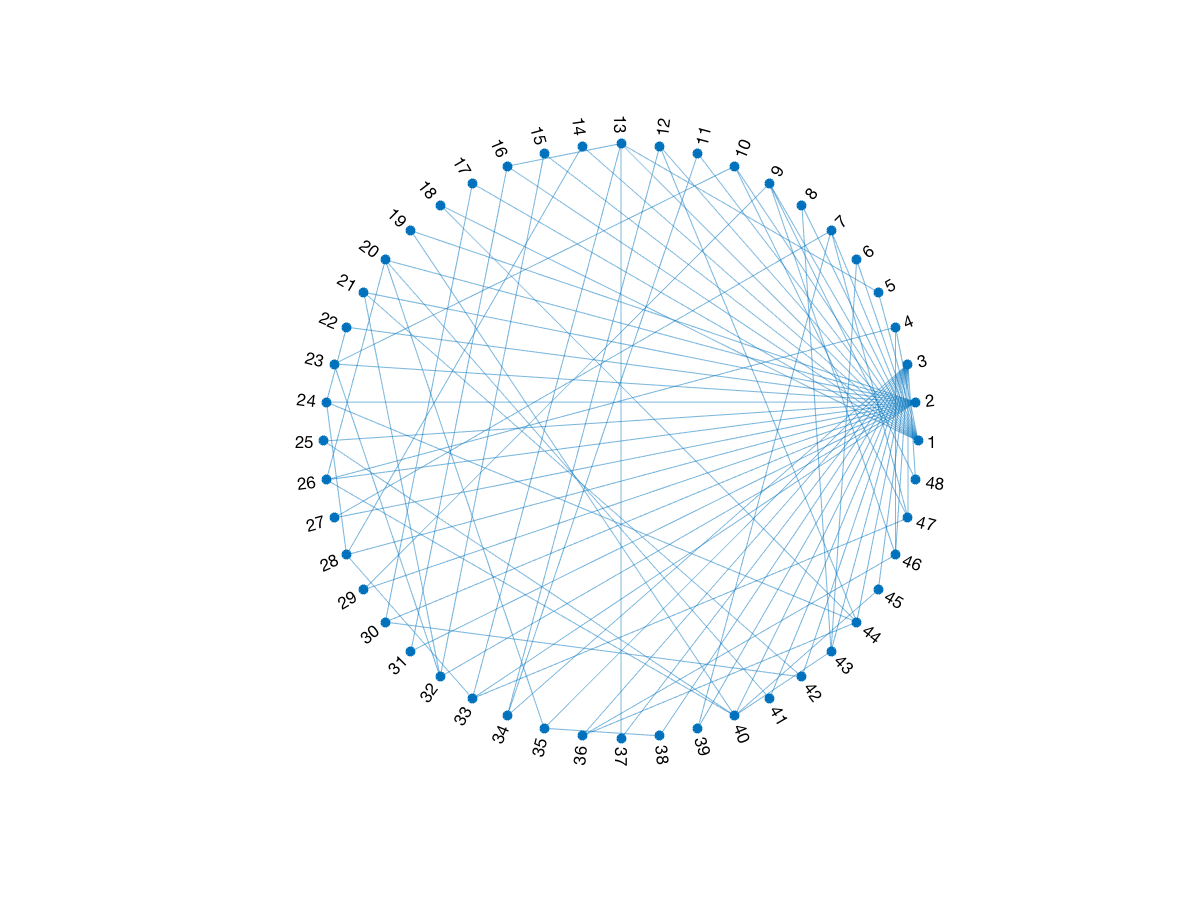
\includegraphics[width=6cm]{fig/disjoint_graph} 
  &   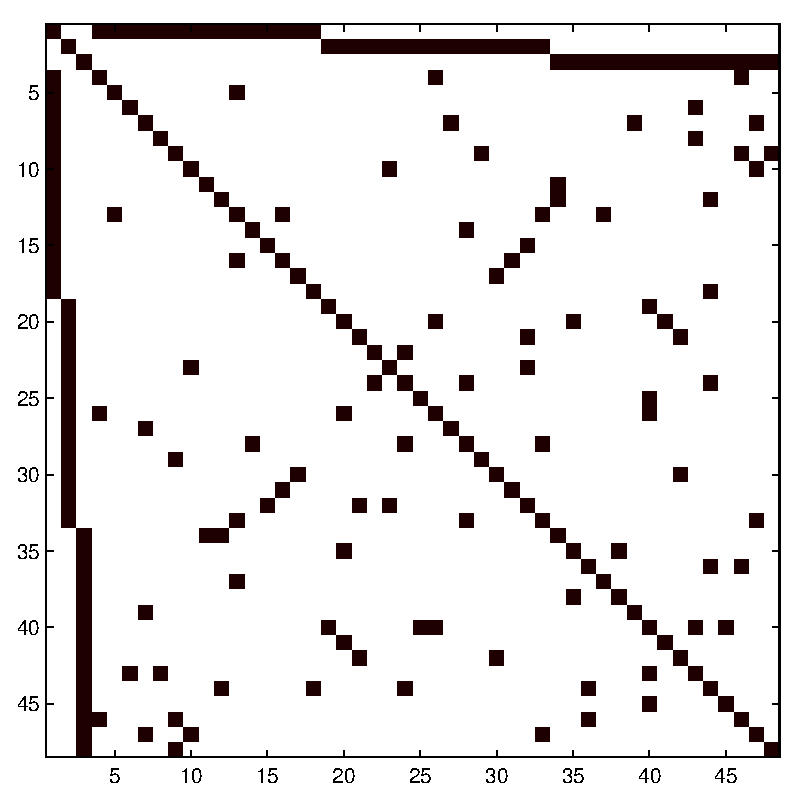
\includegraphics[width=3.5cm]{fig/disjoint_true}
   \\    (a) \textit{model 1} & (b)  structure of concentration matrix for \textit{model 1} \\
      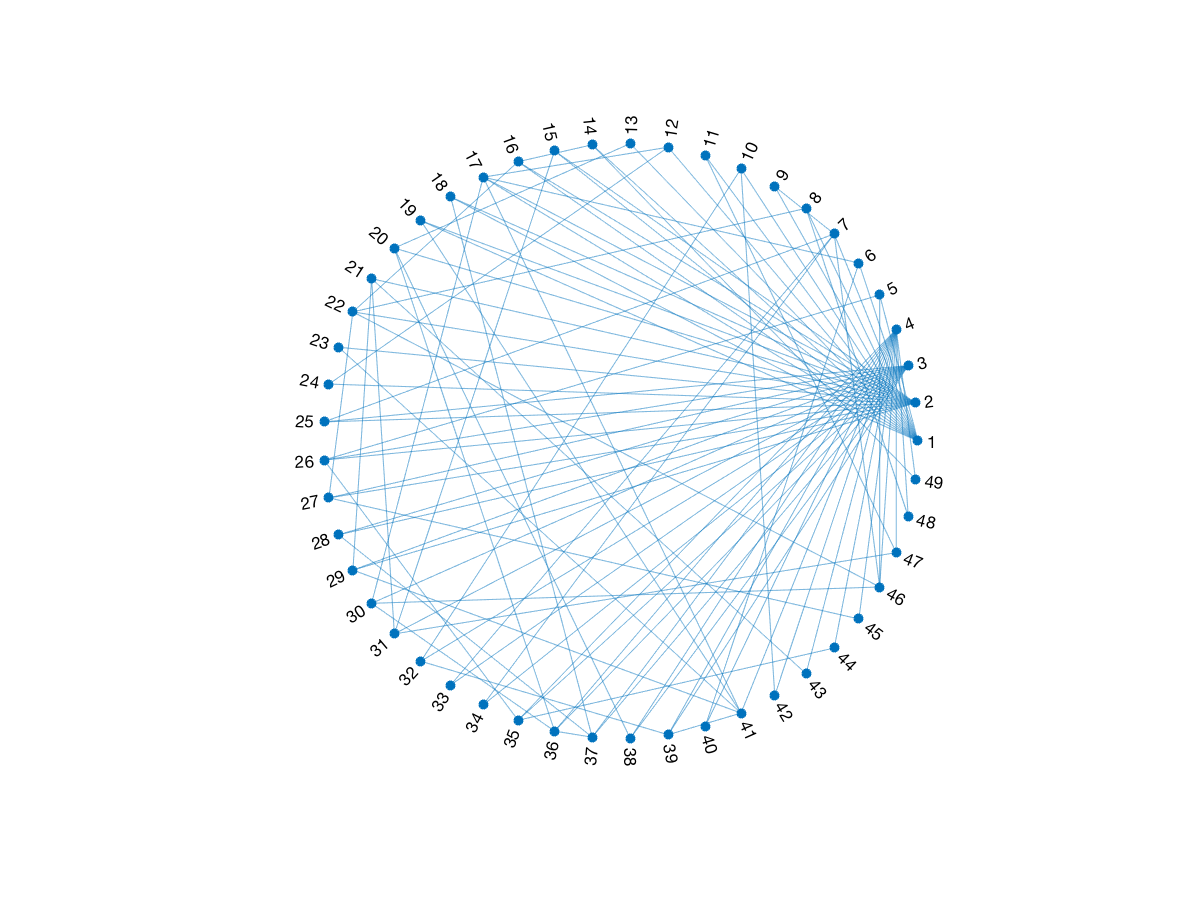
\includegraphics[width=6cm]{fig/over_graph} 
  &   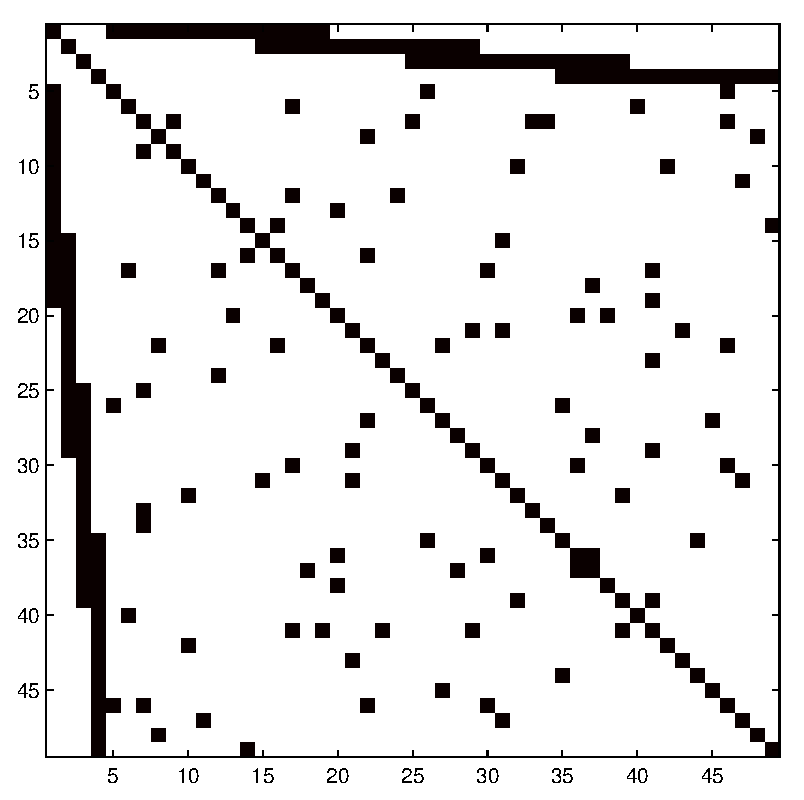
\includegraphics[width=3.5cm]{fig/overlap_true}
   \\    (c) \textit{model 2} & (d)  structure of concentration matrix for \textit{model 2} \\
      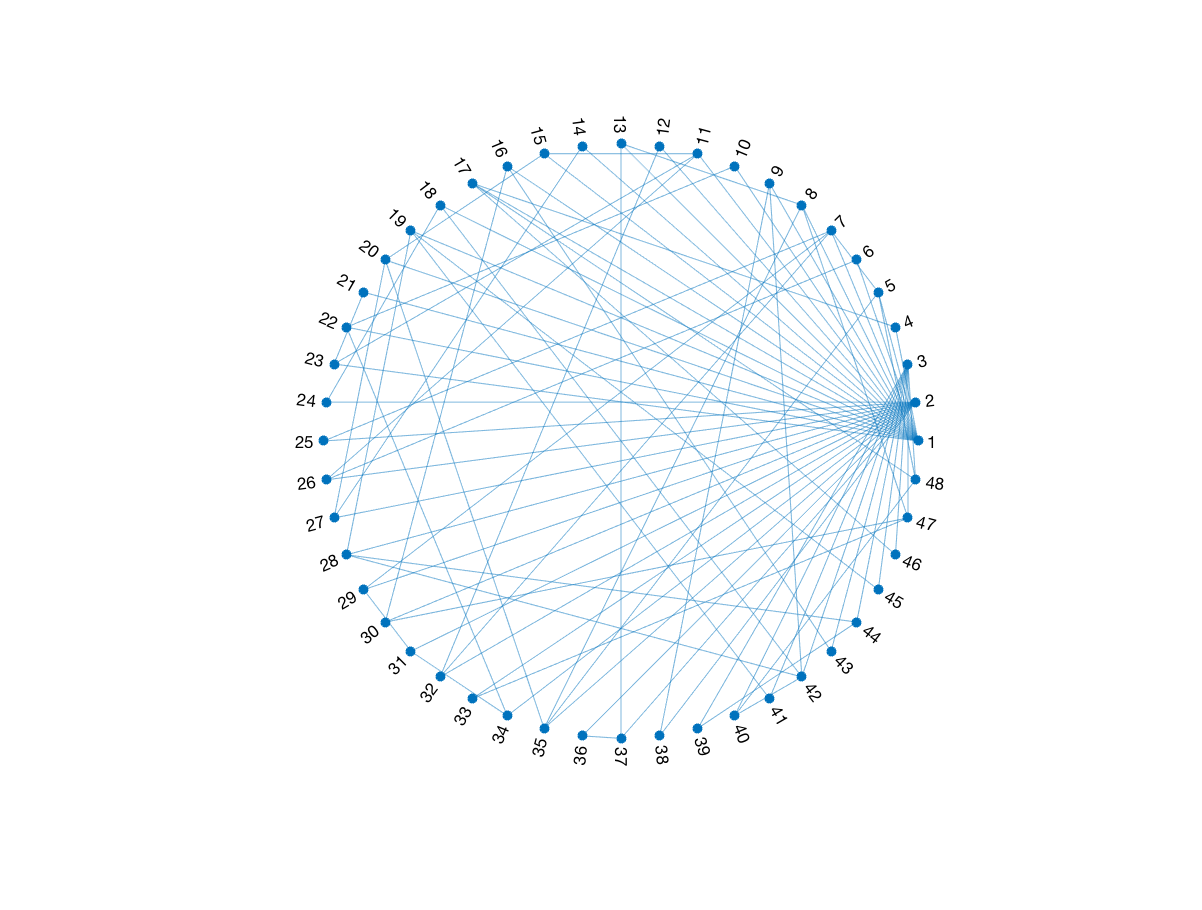
\includegraphics[width=6cm]{fig/diff_graph} 
  &   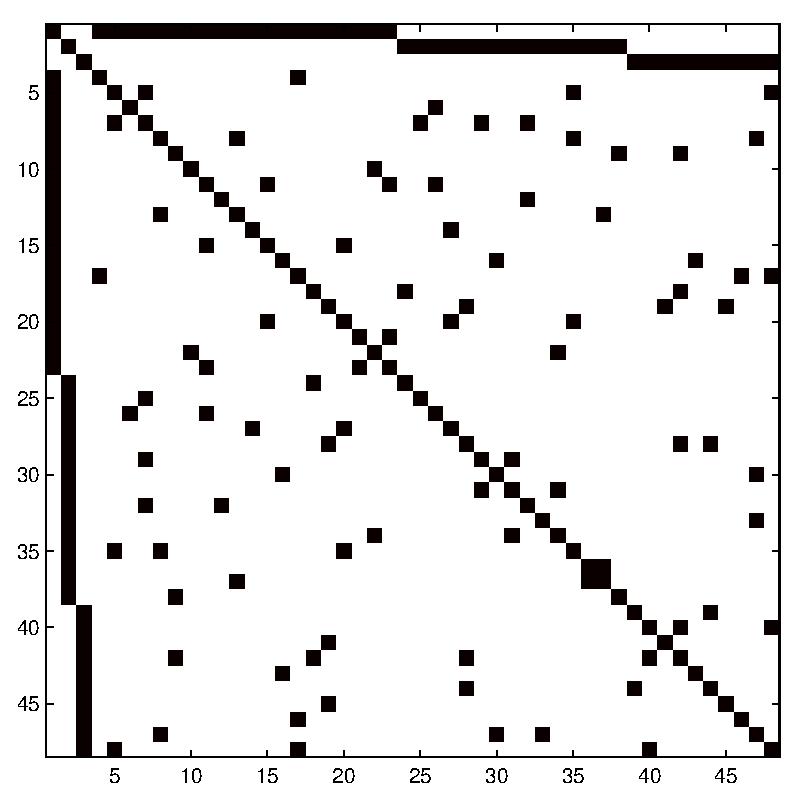
\includegraphics[width=3.5cm]{fig/diff_true}
   \\    (e) \textit{model 3} & (f)  structure of concentration matrix for \textit{model 3}
\end{tabular}
\caption{ Structures of graphical models for the synthetic experiments}
\end{figure}

\begin{figure}
\center
\begin{tabular}{cccc}
      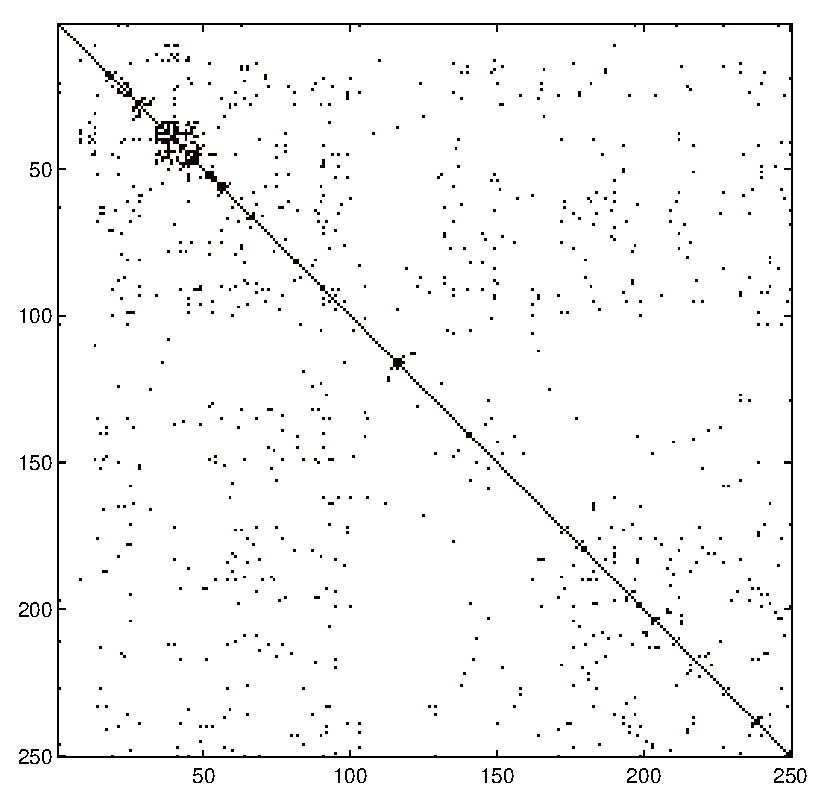
\includegraphics[width=4cm]{fig/MILE_Som}
  &   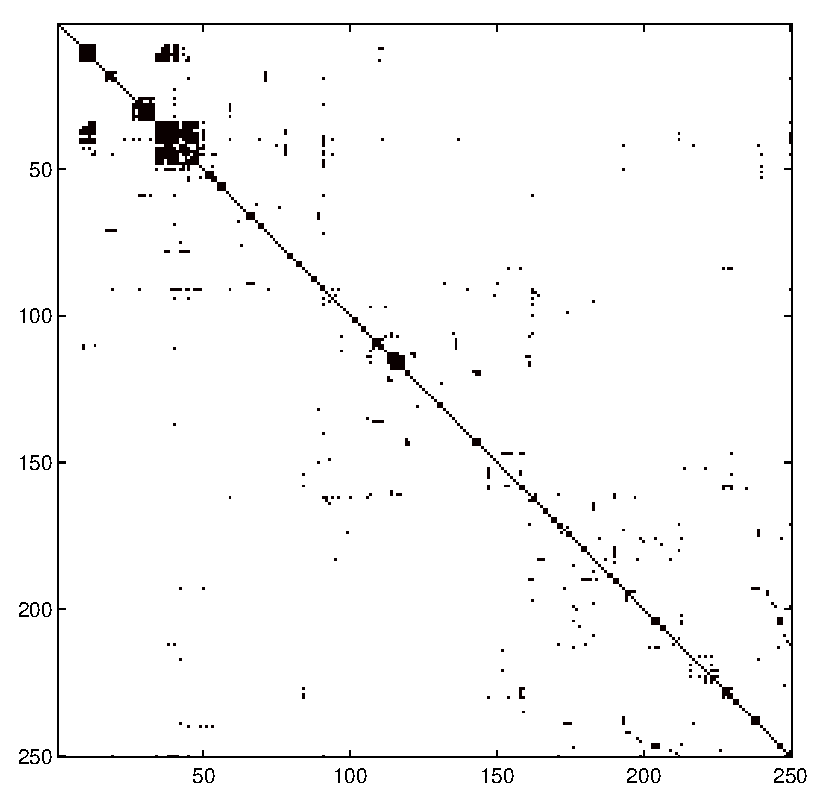
\includegraphics[height=3.8cm]{fig/MILE_Ssl_ordered}
   \\   (a)  $\hat{S}$ $\ell_1+\tr$  & (b) $\hat{S}$ ours 
\end{tabular}
\caption{Sparse component for our method (a) for maximum log-likelihood regularized by $\ell_1+\tr$ (b) }
\end{figure}

\end{document}

%\section*{References}
\bibliographystyle{apalike}
\bibliography{lvggm}